
Image generative modeling saw drastic quality improvement with the advent of text-to-image diffusion models~\cite{Rombach_2022_CVPR} trained on billion-scale datasets~\cite{schuhmann2022laion} with large parameter counts~\cite{peebles2023scalable}. 
%
From a short prompt, these models generate photorealistic images, 
with strong zero-shot generalization to new classes~\cite{li2023your}.
%
Efficient training methods for image data, combined with Internet-scale datasets, enabled the development of these models. However, applying similar techniques to domains where huge datasets are scarce, such as 3D shape generation, remains challenging.

The need for 3D objects in downstream applications like vision, graphics, and robotics motivated methods like Score Distillation Sampling (SDS)~\cite{poole2022dreamfusion} and Score Jacobian Chaining (SJC)~\cite{wang2023score}, which optimize volumetric 3D representations~\cite{mildenhall2020nerf, muller2022instant, kerbl20233d} using queries to a 2D generative model~\cite{earle2024dreamcraft}.
%
In every iteration, SDS renders the current state of the 3D representation from a random viewpoint, 
adds noise to the result, and then denoises it using the pre-trained 2D diffusion model conditioned on a  text prompt. 
%
The difference between the added and predicted noise is used as a gradient-style update on the rendered images,
which is propagated to the parameters of the 3D model.
%
The underlying 3D representation helps make the generated images multi-view consistent,
and the 2D model guides individual views towards a learned distribution of realistic images.



In practice, however, as noted in~\cite{wang2024prolificdreamer, katzir2023noise, zhu2023hifa}, 
SDS often produces 3D representations with over-saturated colors and over-smoothed textures (\cref{fig:teaser}d), not matching the quality
of the underlying 2D model. 
%
Existing approaches tackling this problem improve quality at the cost of expensive re-training or fine-tuning of the image diffusion model~\cite{wang2024prolificdreamer}, complex multi-stage handling of 3D representations like mesh extraction and texture fine-tuning~\cite{lin2023magic3d, tang2023make, wang2024prolificdreamer}, or altering the SDS guidance~\cite{zhu2023hifa, katzir2023noise, yu2023text}.
%


\begin{figure}[t]
    \centering
    %\vspace{-.1in}
    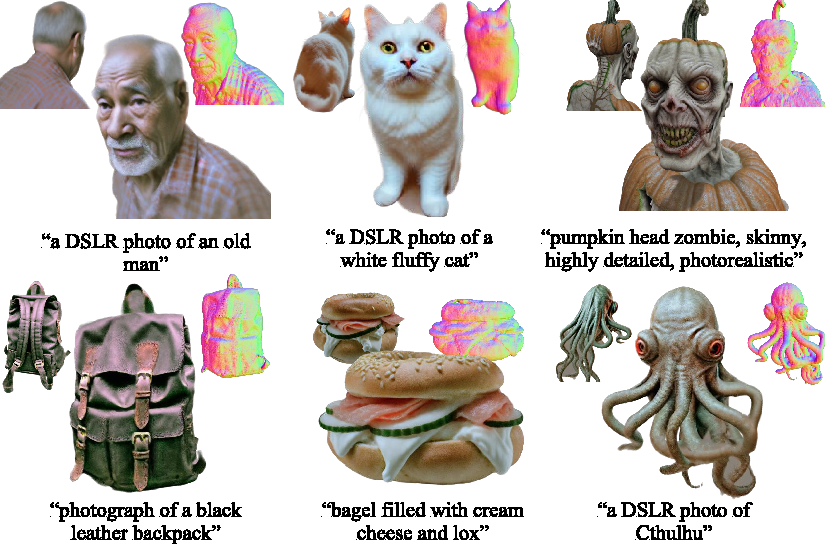
\includegraphics[width=0.99\linewidth]{figs/main_ours_results.pdf}
    \vspace{-.0 in}
    \caption{Examples of 3D objects generated with our method.\vspace{-.25 in}}
    \vspace{-.1 in}
    \label{fig:main_ours_results}
\end{figure}

As an alternative to engineering-based improvements to SDS, in this paper we reanalyze the vanilla SDS algorithm to understand the underlying source of artifacts. 
%
Our key insight is that the SDS update rule steps along an approximation of the DDIM velocity field.
In particular, we derive Score Distillation from DDIM with a change of variables to the space of single-step denoised images.  
%
In this light, SDS updates are nearly identical 
to DDIM updates, apart from one difference: while DDIM samples noise \textit{conditionally} on the 
previous predictions, SDS resamples noise i.i.d.\ in every iteration.
%
This breaks the denoising trajectory for each independent view and 
introduces excessive variance. 
%
Our perspective unifies DDIM and SDS and 
helps explain why SDS can produce blurry and over-saturated results:
the variance-boosting effect of noisy guidance is usually mitigated with high Classifier-Free Guidance (CFG)~\cite{ho2022classifier} 
to reduce sample diversity at the cost of over-saturation~\cite{lin2024common}.


Based on our analysis, we propose an alternative score distillation algorithm dubbed Score Distillation via Inversion (\ourmethod), 
closing the gap to DDIM.
We obtain the conditional noise required for consistency of the denoising trajectories 
by inverting DDIM on each step of score distillation (\cref{fig:system}).
%
This modification yields 3D objects with high-quality textures consistent with the 2D diffusion model (\cref{fig:teaser}e). 
%
Moreover, in 2D, our method closely approximates 
DDIM while preserving the incremental generation schedule of SDS (\cref{fig:teaser}c). 

Our key contributions are as follows:
{\allowdisplaybreaks
\begin{itemize}
    \item We prove that guidance for each view in the SDS algorithm is a simplified reparameterization of DDIM sampling: vanilla SDS samples random noise at each step, while DDIM keeps the trajectories consistent with previously-predicted noise.
    \item We propose a new method titled Score Distillation via Inversion (SDI), which replaces the problematic random noise sampling in SDS with 
    prompt-conditioned DDIM inversion and significantly improves 3D generation,
    closing the quality gap to samples from the 2D  model.
    \item We systematically compare \ourmethod ~with the state-of-the-art Score Distillation algorithms and show that SDI achieves similar or better generation quality, while not requiring training additional neural networks or multiple generation stages.
 \end{itemize}
}

